\section{Evaluation}
\label{sec:evaluation}

We now evaluate the data transfer overhead in the context of cloud-based
autonomous driving.
We assume that autonomic control and environmental perception are
provided in the remote server, but they are not within the scope of this
paper.
What we focus on in this experiment is the measurement of the data
transfer overhead.
Throughout the experiment, we assume that WiFi (IEEE802.11n
2.4GHz/5.0GHz) is provided with bandwidth of 300Mbps while LTE (au
2.1GHz LTE) achieves 75Mbps for downstream and 25Mbps for upstream.

\subsection{Control Command Transfer}

This experiment measures the transfer time taken to send control
commands to the vehicle from a smartphone.
The commands control the steering, accelerator, and brake of the vehicle.
The steering angle is determined by the gyro sensor data while the
accelerator and break strokes are manipulated by the graphics user
interface of the Andrive application.
We use an HTC J butterfly Snapdragon S4 Pro (APQ8064@1.5GHz, Quad Core)
smartphone for a testing terminal.

\begin{figure}[!t]
 \centering
 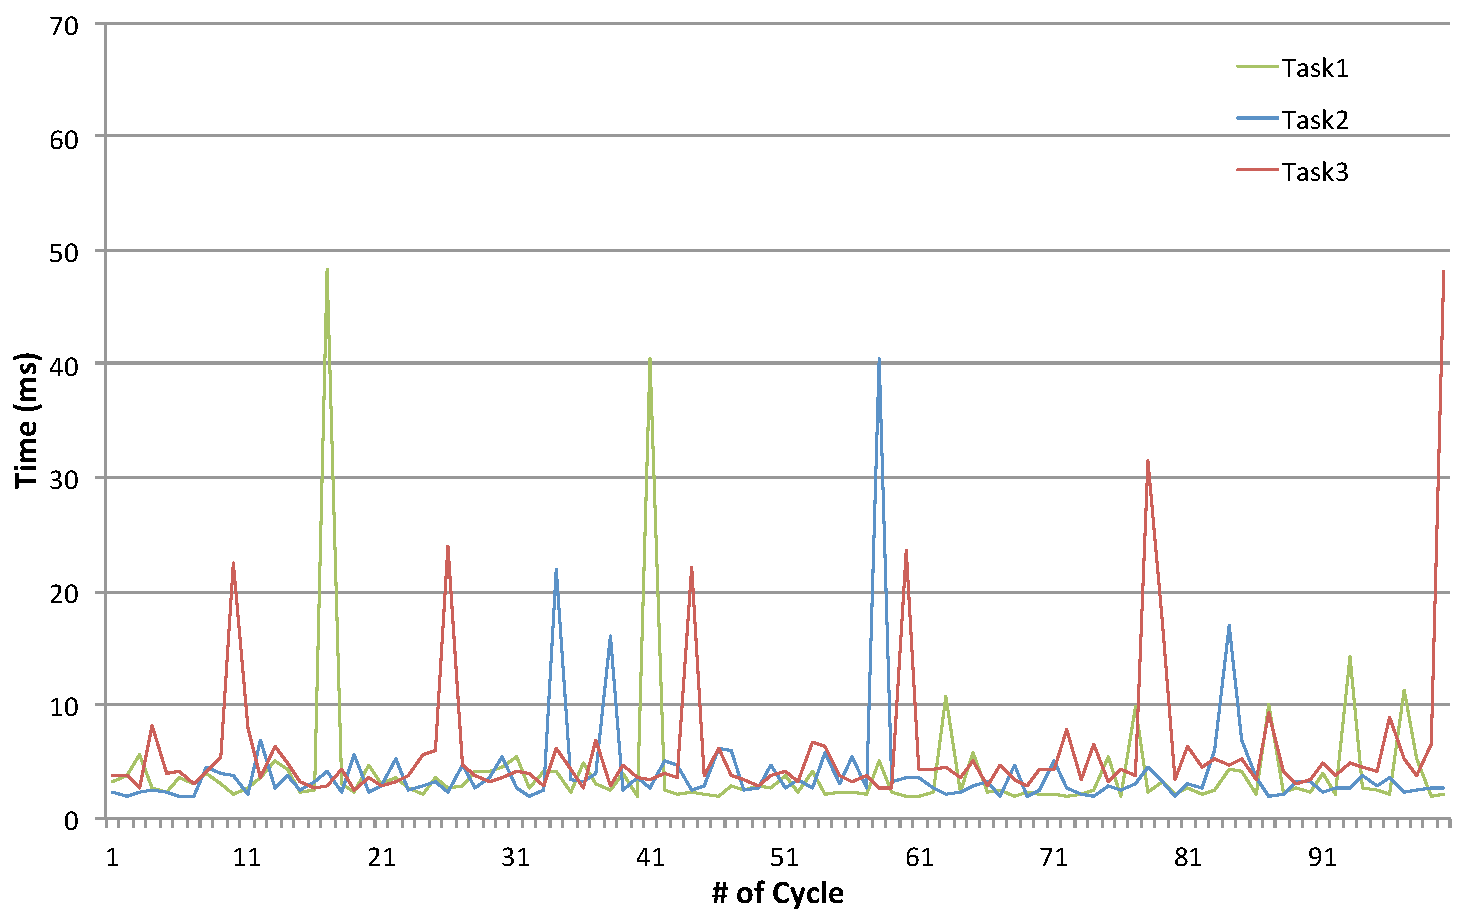
\includegraphics[width=0.8\hsize]{fig/No1_Andrive_serv_cycle_WiFi.pdf}
 \caption{The achieved period of \textit{synchronous} data transfers for
 control commands using WiFi.}
 \label{fig:no1}
 \vspace{1em}
 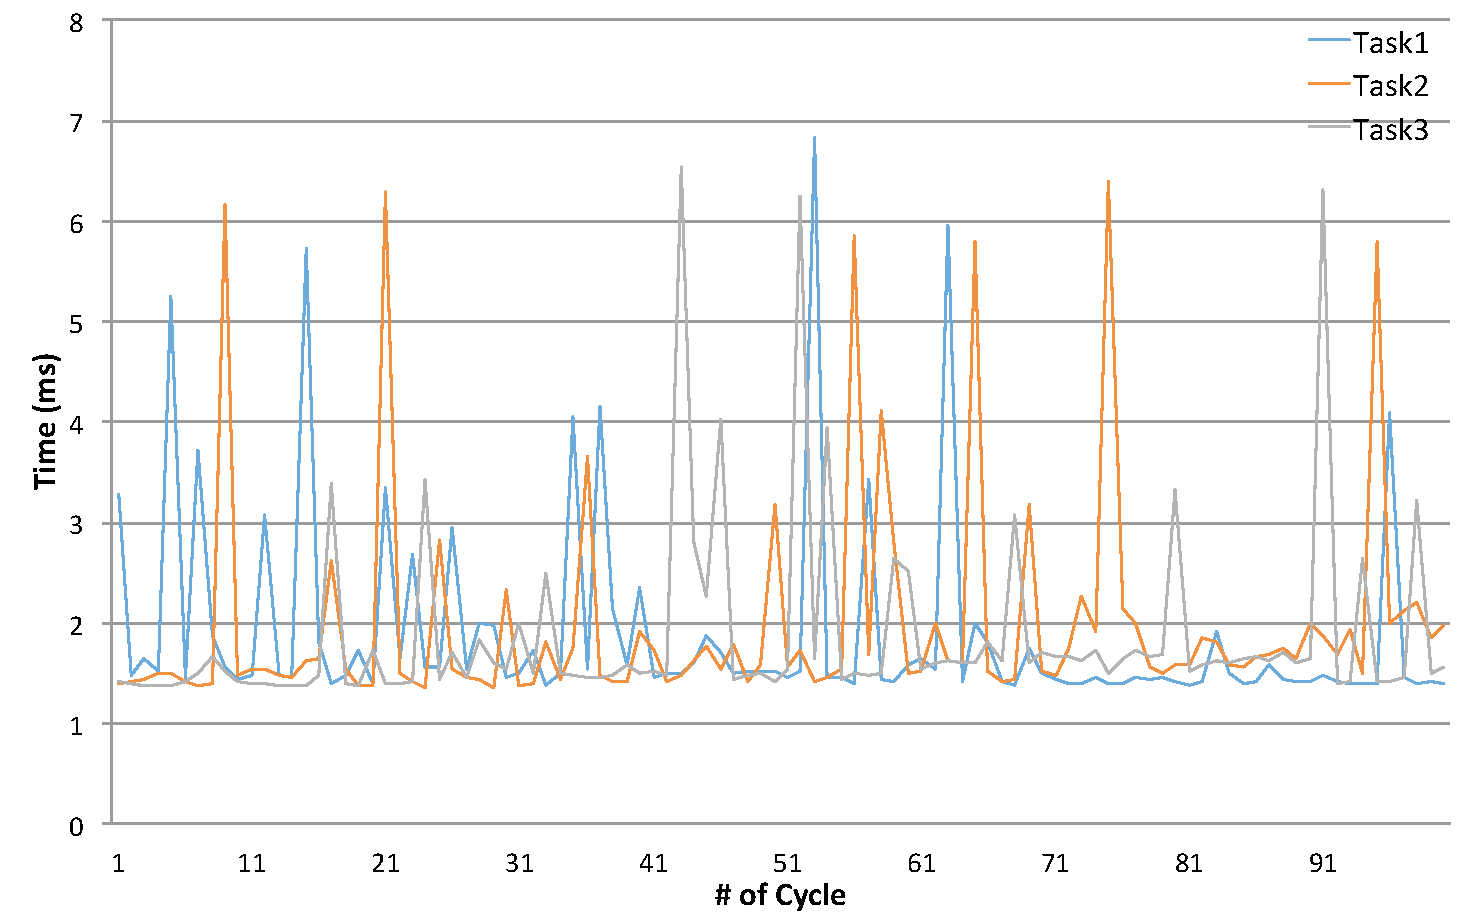
\includegraphics[width=0.8\hsize]{fig/No4_Andrive_serv_cycle_WiFi_only_send.pdf}
 \caption{The achieved period of \textit{asynchronous} data transfers
 for control commands using WiFi.}
 \label{fig:no4}
\end{figure}

Fig. \ref{fig:no1} shows the period (interarrival time) of data
transfers for vehicle control commands achieved using WiFi when the
vehicular master computer in the vehicle and a client smartphone are
synchronized.
The nodes are connected within a local area network, and the vehicular
master computer sends back an acknowledgment message to the smartphone
every time the commands are received for synchronization.
The results after a few seconds from an establishing connection between the smartphone and the server are not included
since the network is unstable after the establishing connection.
It meets a period of $2ms$ on average, which is acceptable for the
feedback control rate of autonomous driving \cite{Kagami13}.
However there are unpredictable spikes that increase the period up to
$7ms$ in the worst case.
These unpredictable spikes are not acceptable under real-time
constraints.

Fig. \ref{fig:no4} shows the period of data transfers in the same
setup as Fig. \ref{fig:no1} except that the vehicular master computer and
the smartphone are not synchronized, \textit{i.e.}, the smartphone is
sending data without waiting for the acknowledgment message from the
vehicular master computer.
It is clear that some spikes are removed as compared to
Fig. \ref{fig:no1}.

\begin{figure}[!t]
 \centering
 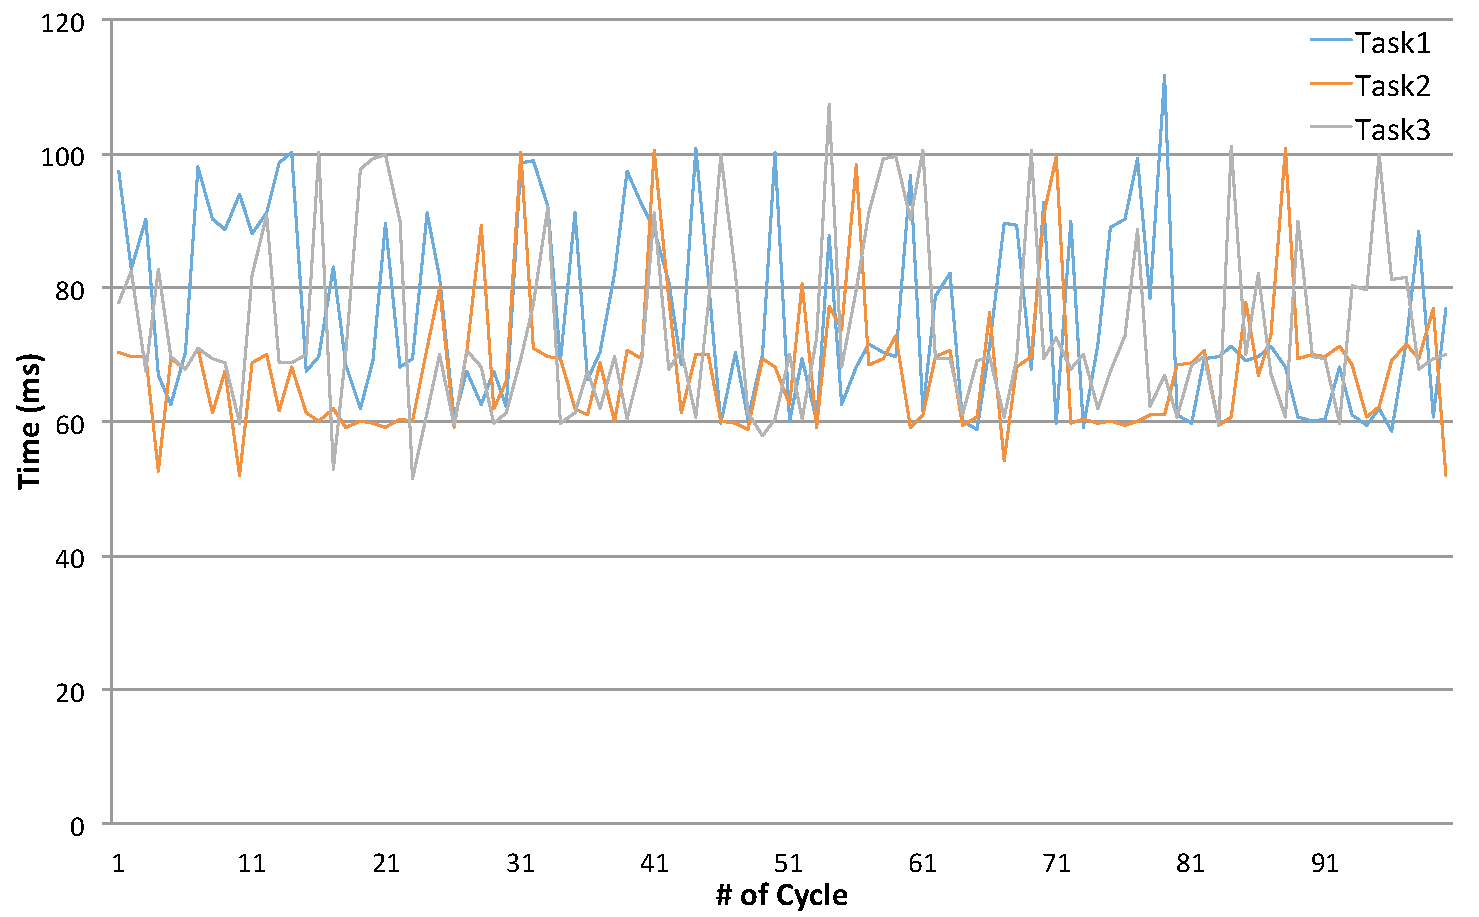
\includegraphics[width=0.8\hsize]{fig/No2_Andrive_serv_cycle_LTE.pdf}
 \caption{The achieved period of \textit{synchronous} data transfers for
 control commands using LTE.}
 \label{fig:no2}
 \vspace{1em}
 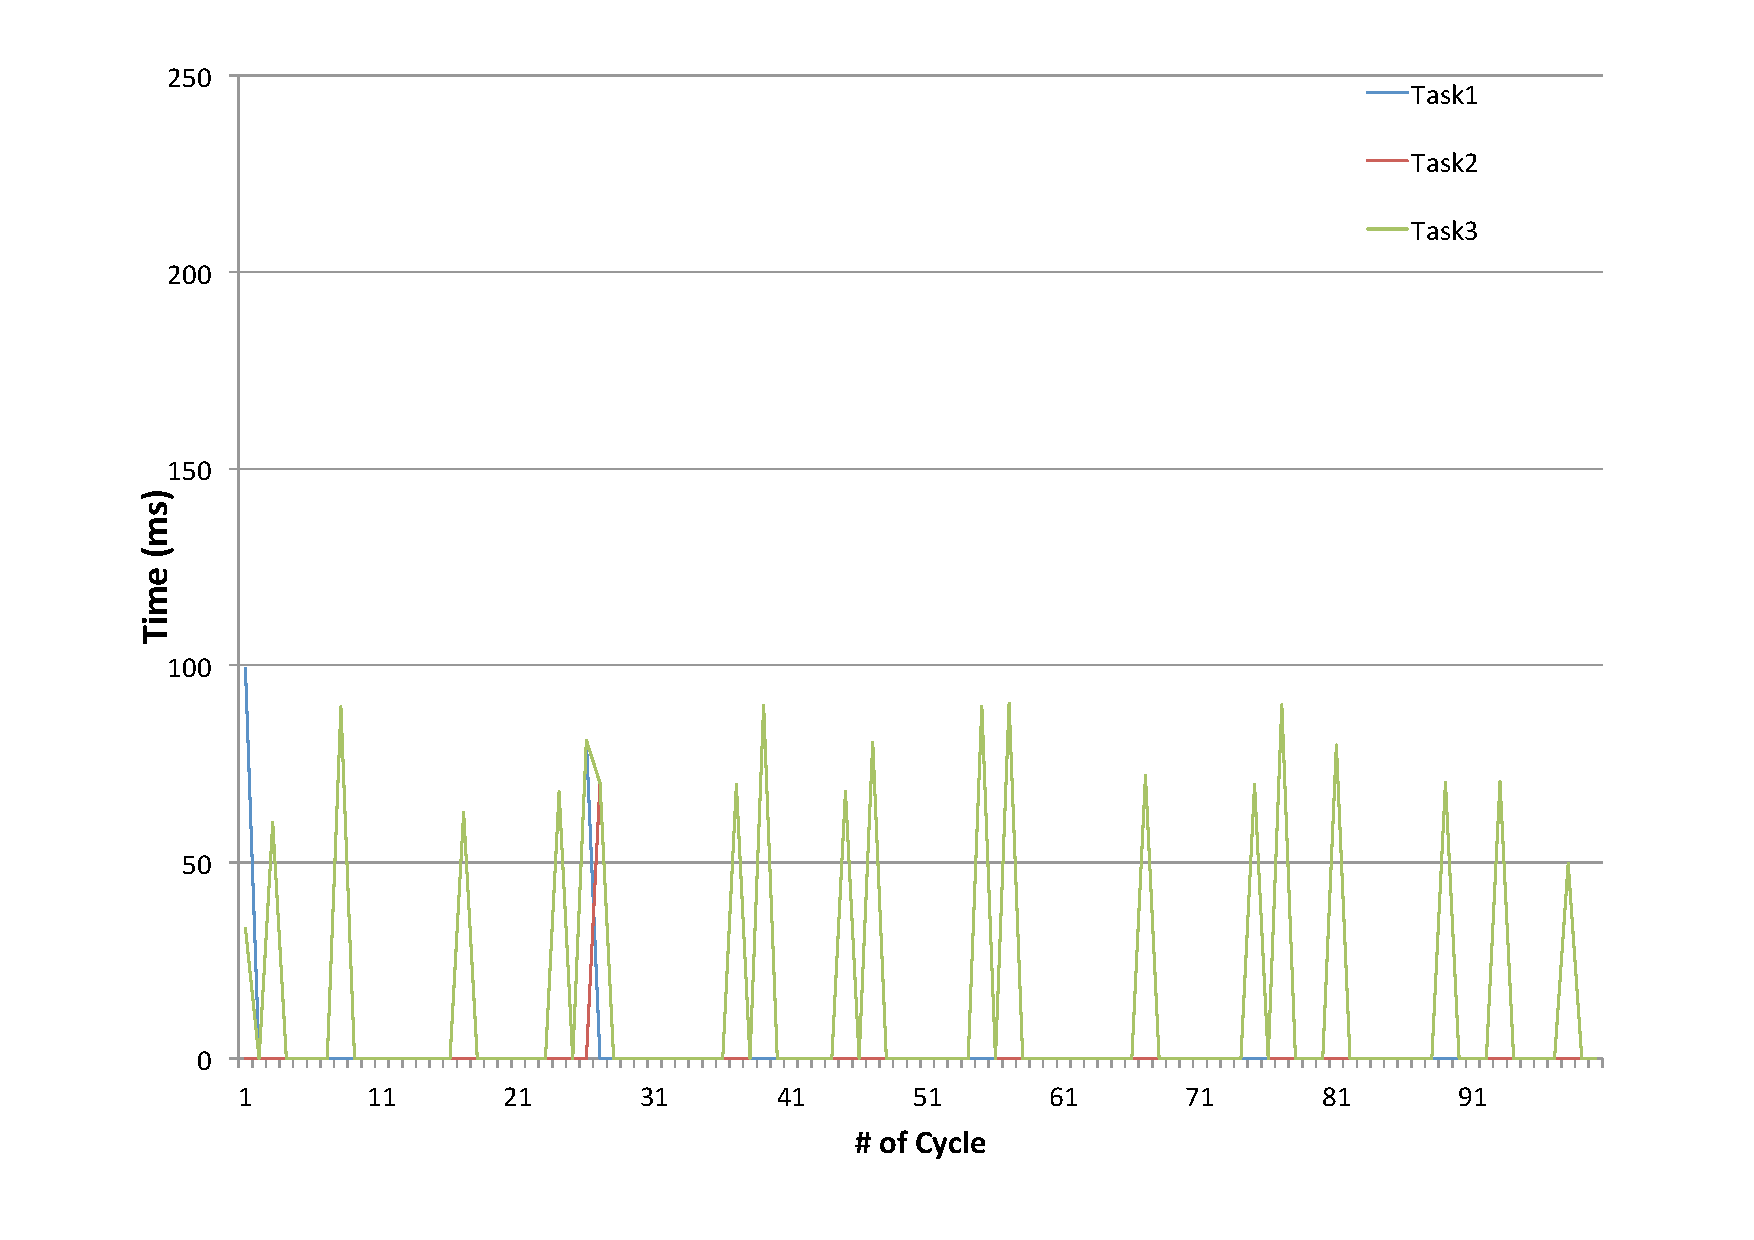
\includegraphics[width=0.8\hsize]{fig/No5_Andrive_serv_cycle_LTE_only_send.pdf}
 \caption{The achieved period of \textit{asynchronous} data transfers for
 control commands using LTE.}
 \label{fig:no5}
\end{figure}

Figs. \ref{fig:no2} and \ref{fig:no5} show the period of data transfers
for the same set of vehicular control commands using LTE.
While WiFi is often suitable for intranet usage, LTE is more publicly
deployed in the city as part of wireless internet services.
As compared to WiFi, the data transfer times achieved by LTE are
increased due to its less bandwidth.
It takes around $100ms$ to transfer a single set of control commands,
and some spike reaches $110ms$ in the worst case when the smartphone
waits for an acknowledgment message from the server for every
transfer.
An asynchronous transfer can mitigate this spike but the average period
of data transfers is still capped at around $100ms$.
In the evaluation environment of LTE, 
the difference between synchronous and asynchronous transfers is only around $10ms$
since downstream (the server to the smartphone) is three times faster than upstream (the smartphone to the sever).

\begin{figure}[!t]
 \centering
 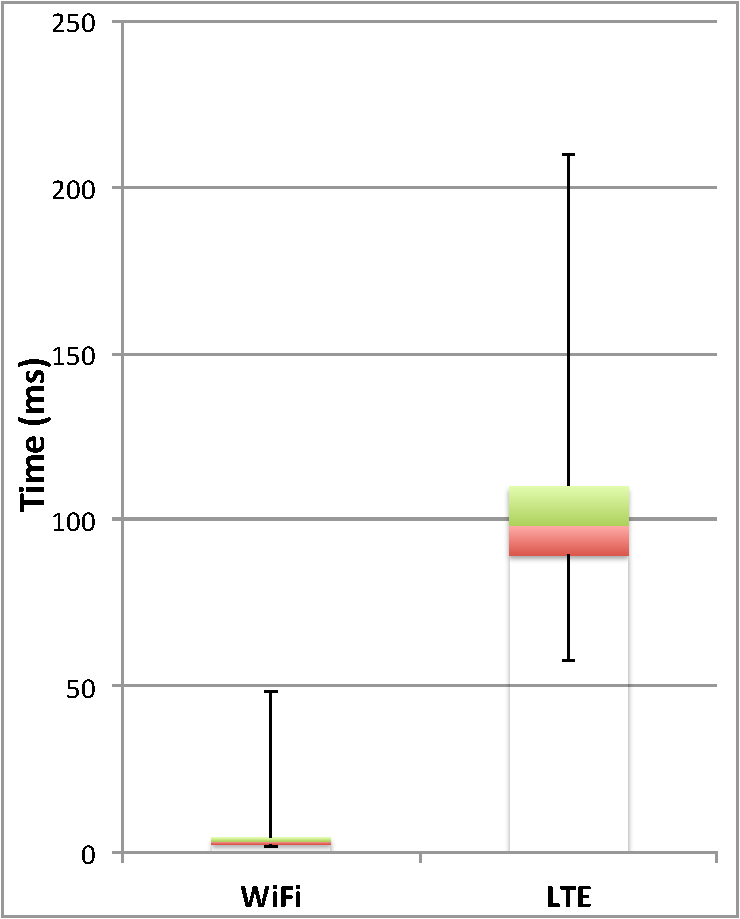
\includegraphics[width=0.45\hsize]{fig/No3_Andrive_boxplot_compare_WiFi_and_LTE.pdf}
 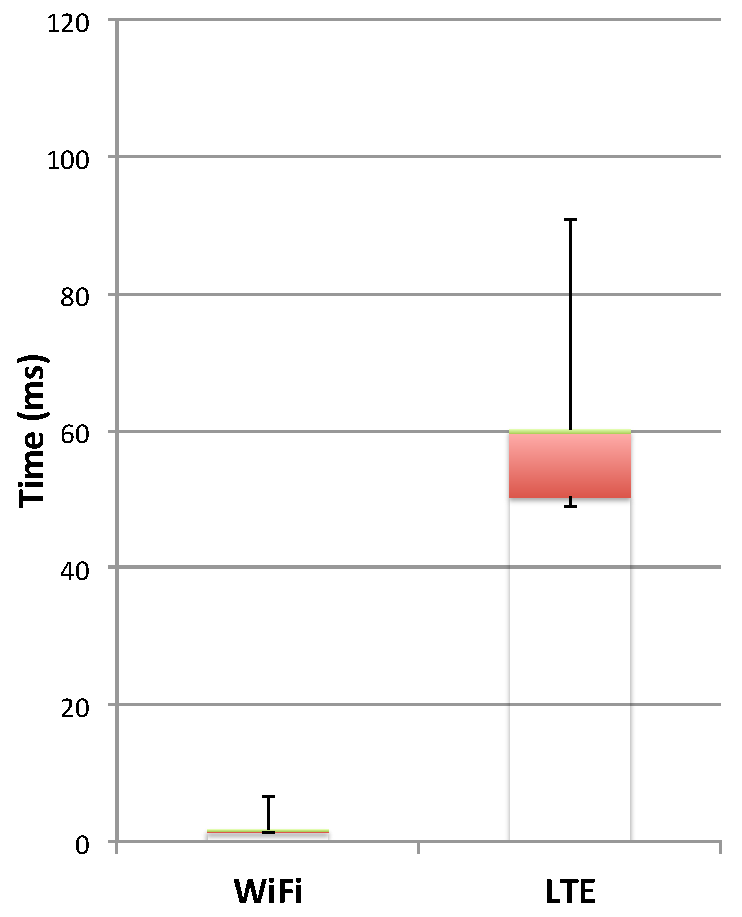
\includegraphics[width=0.45\hsize]{fig/No7_Andrive_only_send_boxplot_compare_WiFi_and_LTE.pdf}
 \caption{Summarized box plotting of the periods for
 \textit{synchronous} (left) and \textit{asynchronous} (right) transfers
 of control commands.}
 \label{fig:no3_7}
\end{figure}

Fig. \ref{fig:no3_7} depicts summarized box plotting of the achieved
data transfer periods for vehicular control commands.
This explains that WiFi is currently a better choice for real-time
communication using commodity ICT platforms.
A significant difference in performance between WiFi and LTE comes from
the fact that LTE is a public service that causes a lot of conflicts
with third people while WiFi used in this setup is a private service
that is dedicated to our experiment of image transfers.
Given this public behavior of LTE, $100ms$ is a reasonable number of the
average period of data transfers for control commands.
We hope that LTE will become more practical for real-time usage as a
publicly available network.

\subsection{Image Transfer}

\begin{figure}[!t]
 \centering
 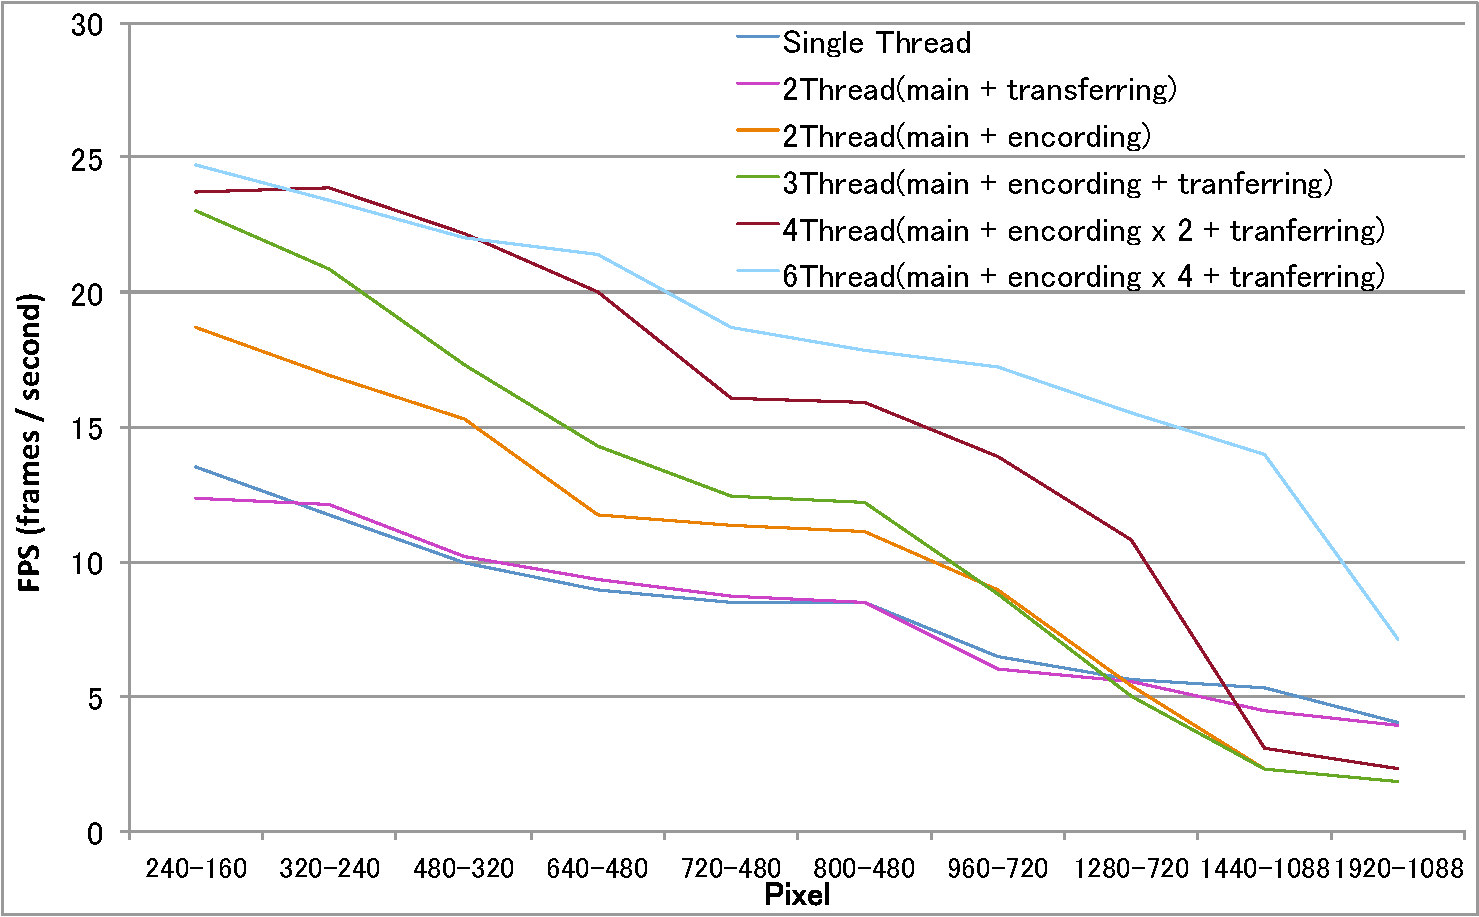
\includegraphics[width=0.8\hsize]{fig/No8_TIPiC_FPS_graph_WiFi.pdf}
 \caption{The frame rate of image transfers using WiFi.}
 \label{fig:no8}
\end{figure}

Fig. \ref{fig:no8} shows the average frame rate of image transfers
achieved using WiFi.
We provide six variants of the image transfer program running on the
smartphone.
As described in Section \ref{sec:prototype}, the throughput of image
transfers can be improved by multithreading.
The top label (Single Thread) uses only a single thread to capture,
encode, and transfer images.
The other labels represent such implementations that use pipelining with
multithreading.
Comparing ``2Threads (main and transferring)''  and ``2Threads (main and encoding)``,
the result shows that the transferring thread is not efficent when the number of encoding threads is small.
Moreover it is speculated that the execution time of the transferring thread is short and finishs during the main thread is waiting for camera capture.
%Fig. \ref{fig:no8}からシングルスレッドと2スレッド(main + transferring)を比較するとエンコードをシングルスレッドで
%行う場合は、あまり効果がないと言える。
%また、シングルスレッドと2Thread(main + transferring)は解像度1440x1088あたりでFPSが2Thread(main + encording), 3Thread, 4Threadと逆転する。この事象は、実装の問題により%発生する。本プログラムは、カメラから取得した画像データをキューに格納しており、そのキューに溜まった画像データをエンコードスレッドが順にエンコードするという形をとる。解像度が大きくなるにつれてエンコードに要する時間は増え、画像データを取得する周期にエンコードスレッドが追いつかなくなる。エンコード処理が追いつかなることによってキューに画像データが溜まり過ぎ、メモリ不足によりパフォーマンス著しく下がることで、この逆転現象が発生している。
Especially the stage of encoding is time consuming, we also use multiple
threads for encoding itself.
In case of more than image size of $1440 \times 1088$ pixels, the single thread is faster than three and four threads.
This performance degradation of three and four threads is due to a shortage of memory of an android application when encoding is much slower than the periods of camera capture. 
However since more than the image size is unusual for smartphone, the problem is not critical in the application.
It is notable that using four or six threads in total, we can meet a
frame rate of more than $20$fps for a standard image size of $640 \times
480$ pixels.
This is a useful finding that we could use smartphones with WiFi to
offload image processing to the cloud in terms of frame rate.

\begin{figure}[!t]
 \centering
 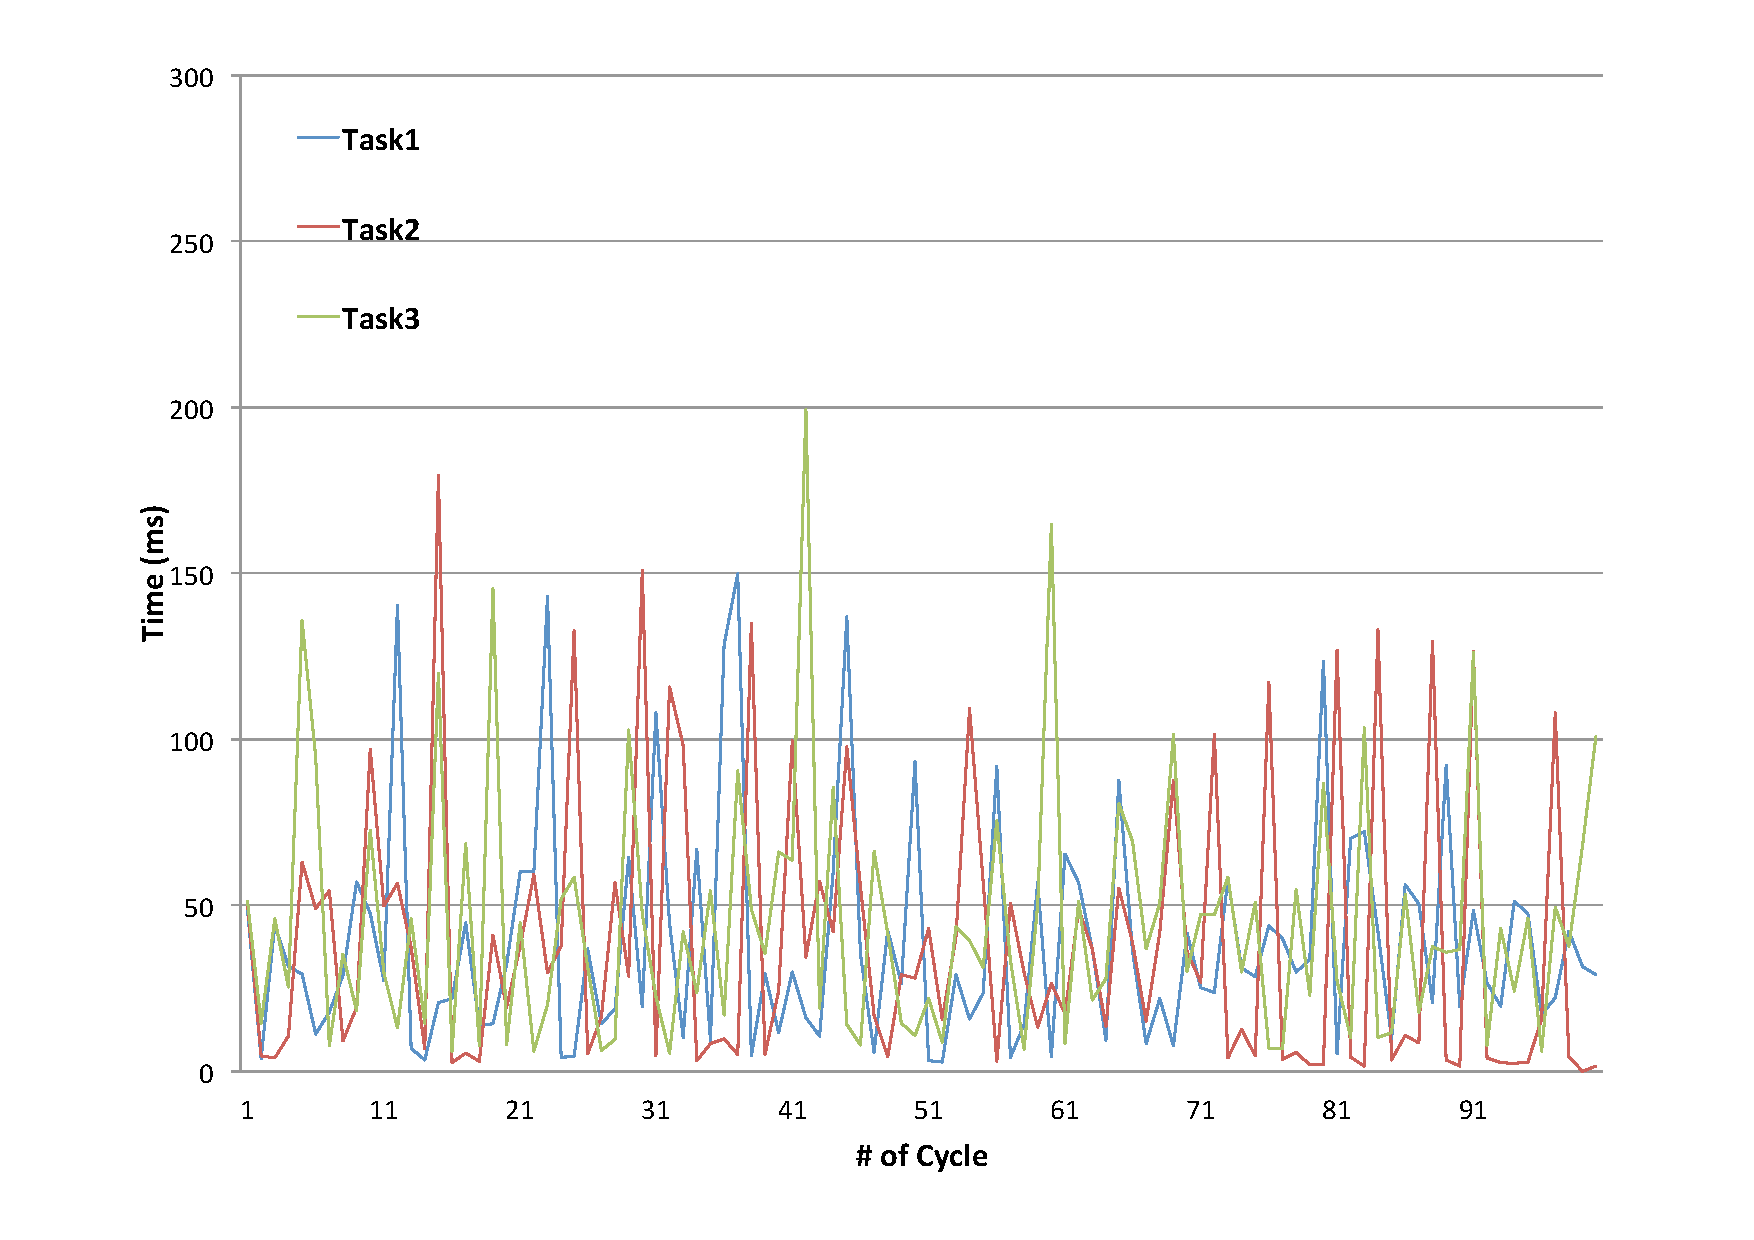
\includegraphics[width=0.8\hsize]{fig/No9_TIPiC_serv_cycle_WiFi.pdf}
 \caption{The achieved period of image transfers using WiFi.}
 \label{fig:no9}
\end{figure}

Henceforth we focus on the best performer of the image transfer program,
\textit{i.e.}, one represented by a label of ``6Threads''.
Fig. \ref{fig:no9} shows the period of image transfers on a cycle basis
achieved using WiFi.
Albeit high frame rates demonstrated in Fig. \ref{fig:no8}, the period is
actually fluctuating to an extent.
For example, some spike reaches $200ms$.
This unpredictable spike may jeopardize fine-grained control that actuates
based on the results of image processing but it also depends on the
algorithm.
From this experiment, therefore, we conclude that the algorithm of
control using the results of networked image processing must be designed
to be dependable against timing jitters.

\begin{figure}[!t]
 \centering
 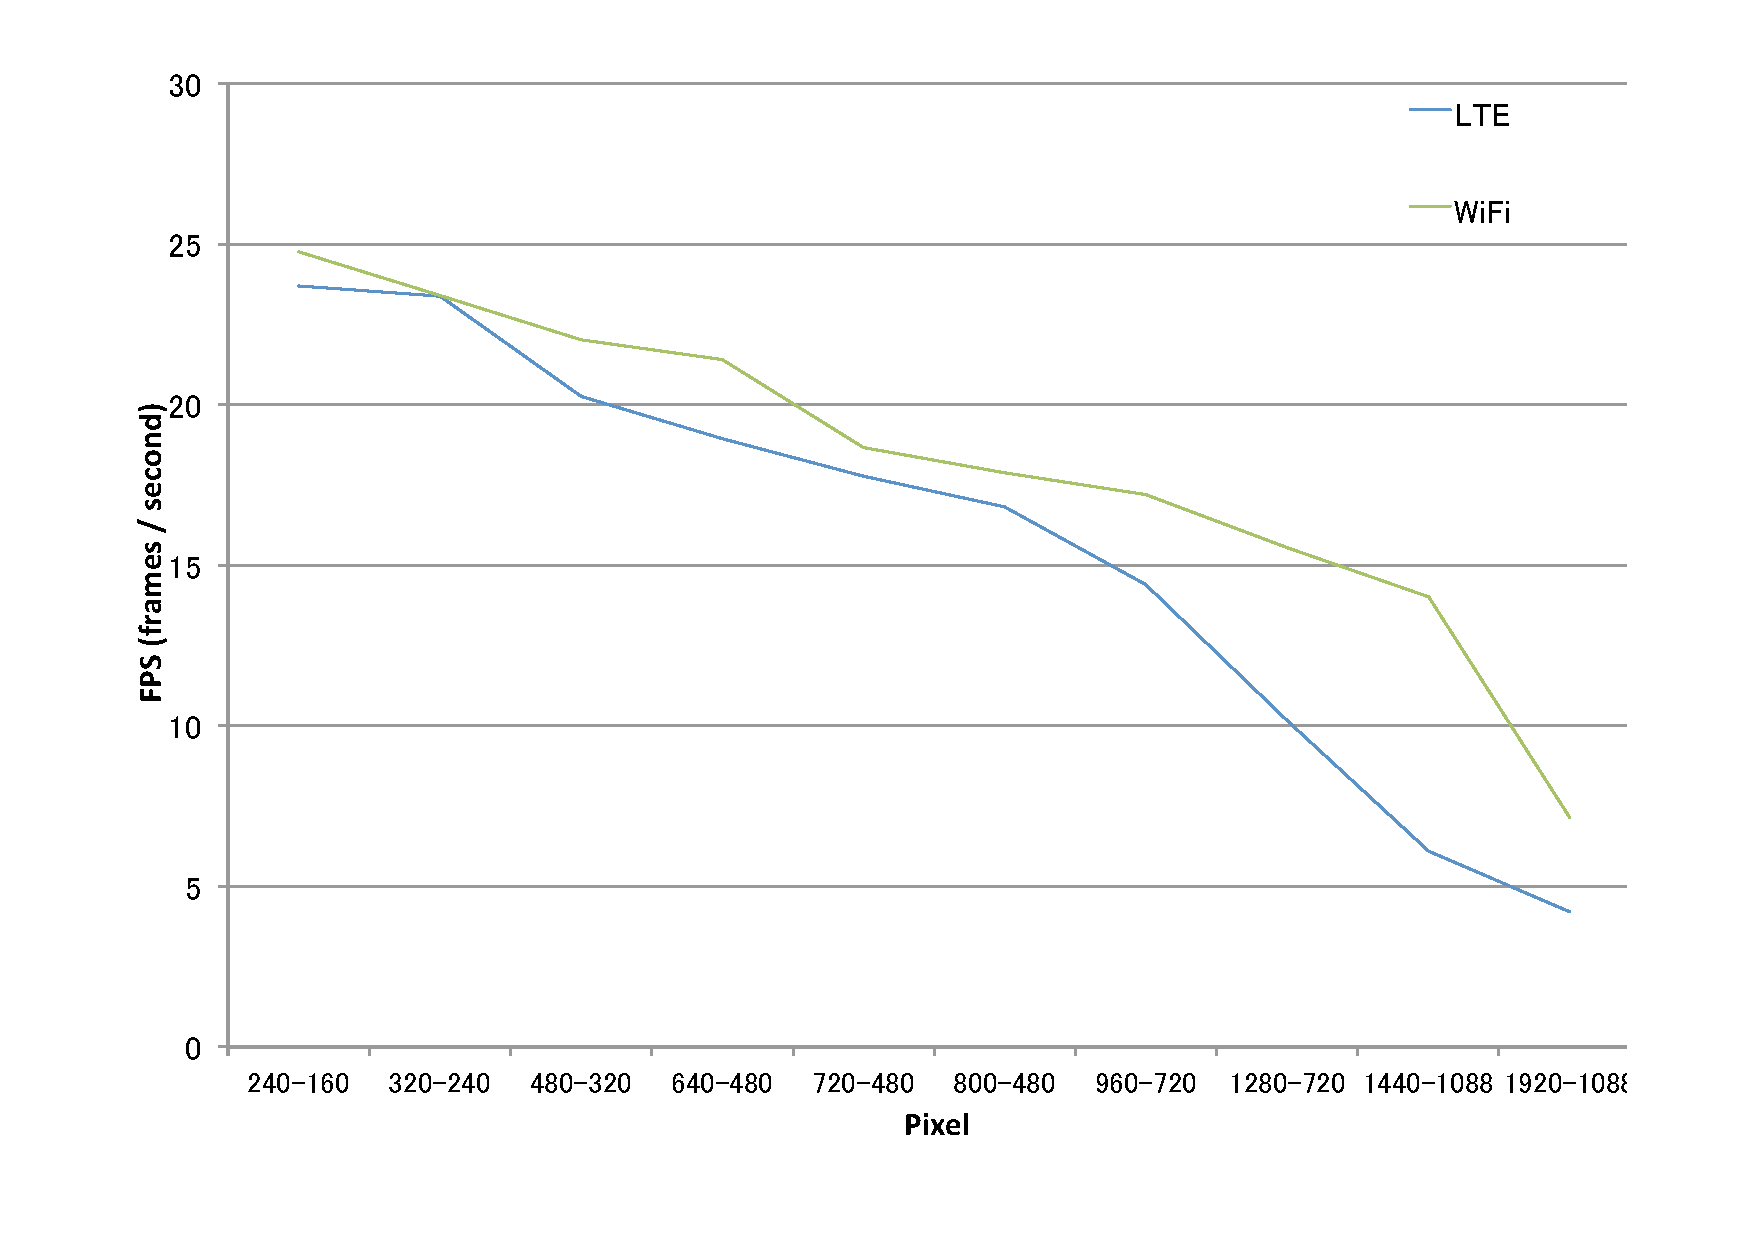
\includegraphics[width=0.8\hsize]{fig/No10_TIPiC_FPS_graph_LTE.pdf}
 \caption{The frame rates of image transfers using WiFi and LTE
 respectively.}
 \label{fig:no10}
\end{figure}

Fig. \ref{fig:no10} shows the frame rate of image transfers achieved
using LTE for the same image set as those shown in Fig. \ref{fig:no8}.
For a reference, the frame rate achieved using WiFi is also plotted.
We omit the variants of the image transfer program other than
``6Threads'', since the observed performance trend is similar to that
shown in Fig. \ref{fig:no8}.
Unlike the previous experiment of control commands highlighting latency,
however, the frame rate of image transfers are not very different
between WiFi and LTE.
Since we use a smartphone employing an embedded processor, we consider
that throughput is more dominated by the processor performance than the
network performance.
This means that LTE is competitive to WiFi in a scenario that we use a
rich smartphone to transfer images to the cloud.

Comparing Figs. \ref{fig:no3_7} and \ref{fig:no10}, in case of LTE,
the results indicates the period of a command (16 bytes) and a small image such as $240\times160$ or $320\times240$ pixels are almost the same.
This means that it takes time to start tranferring data in the LTE enviroment.

\begin{comment}
\begin{figure}[!t]
 \centering
 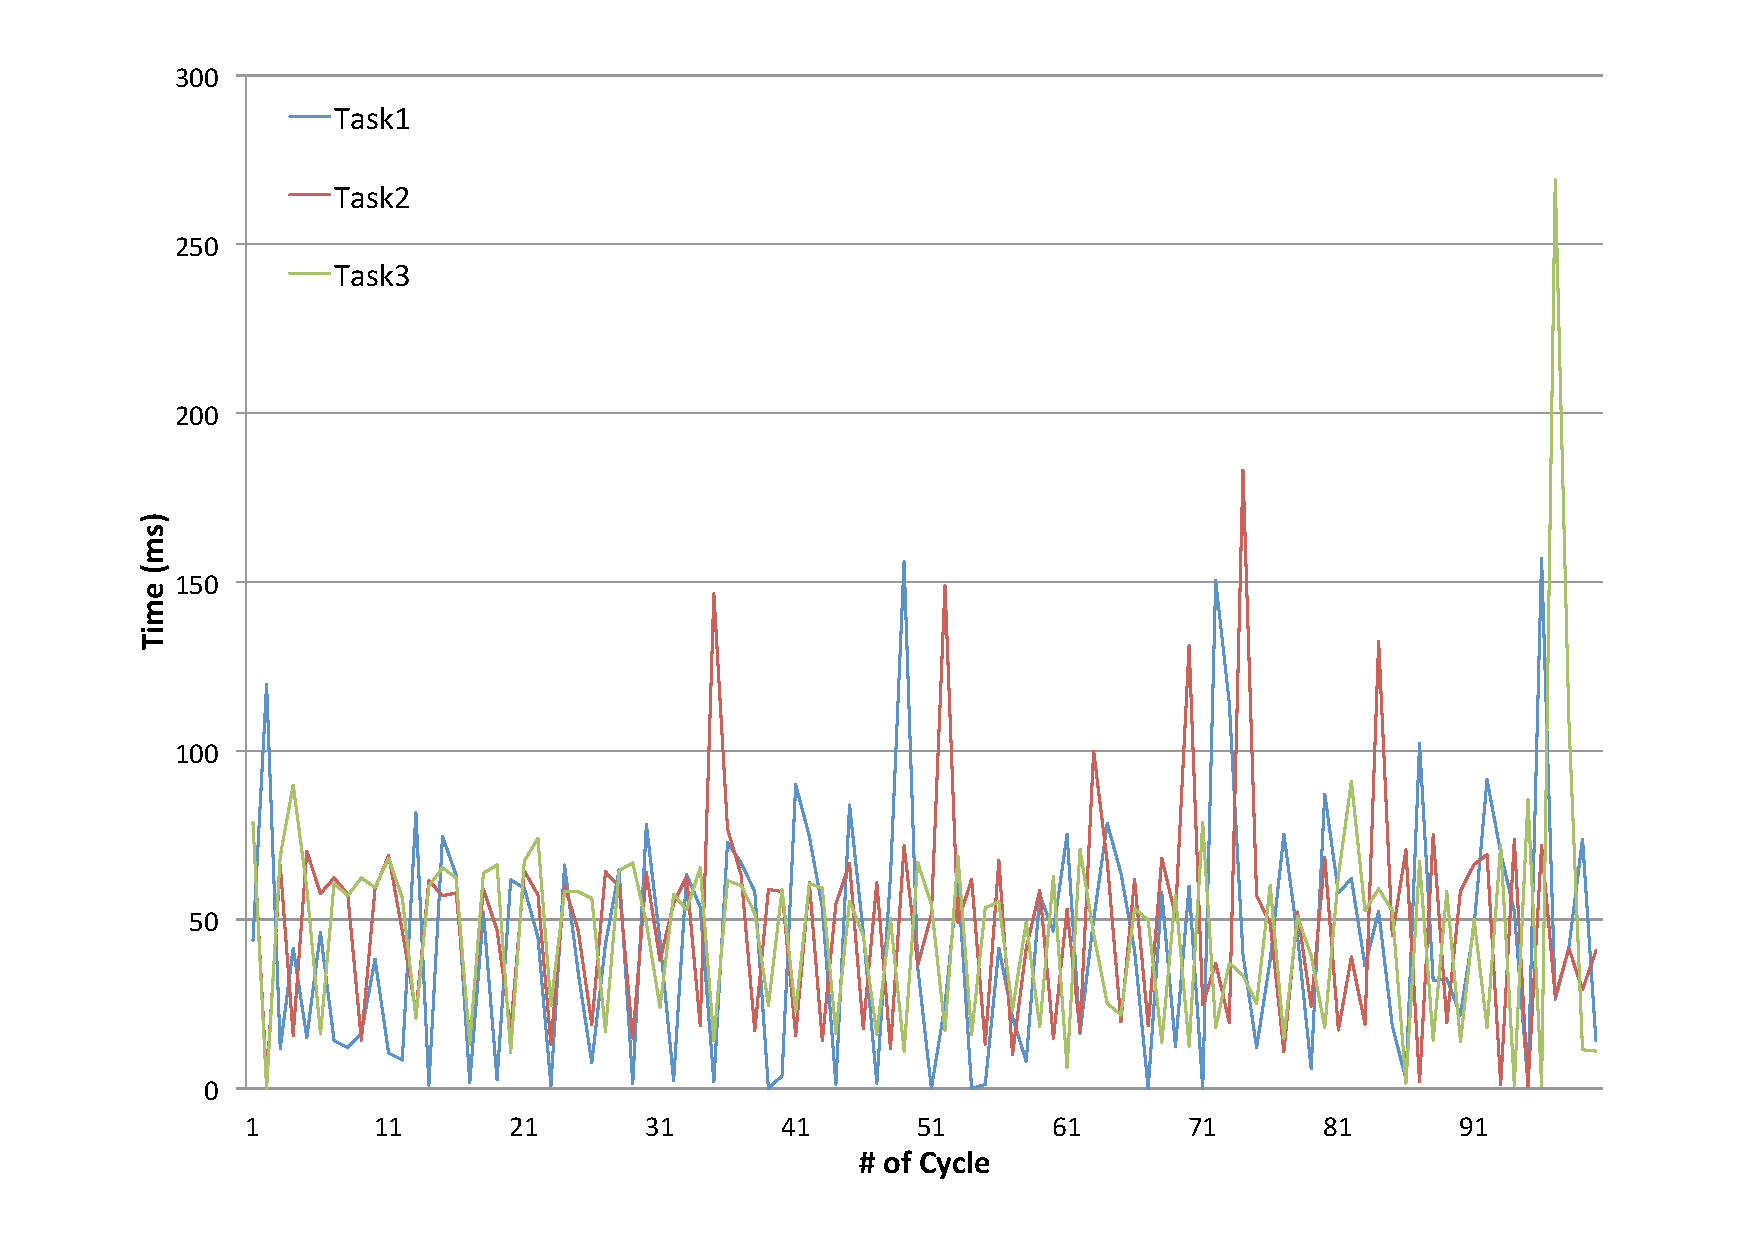
\includegraphics[width=0.8\hsize]{fig/No11_TIPiC_serv_cycle_LTE.pdf}
 \caption{The achieved period of image transfers using LTE.}
 \label{fig:no11}
\end{figure}
\end{comment}

\begin{figure}[!t]
 \centering
 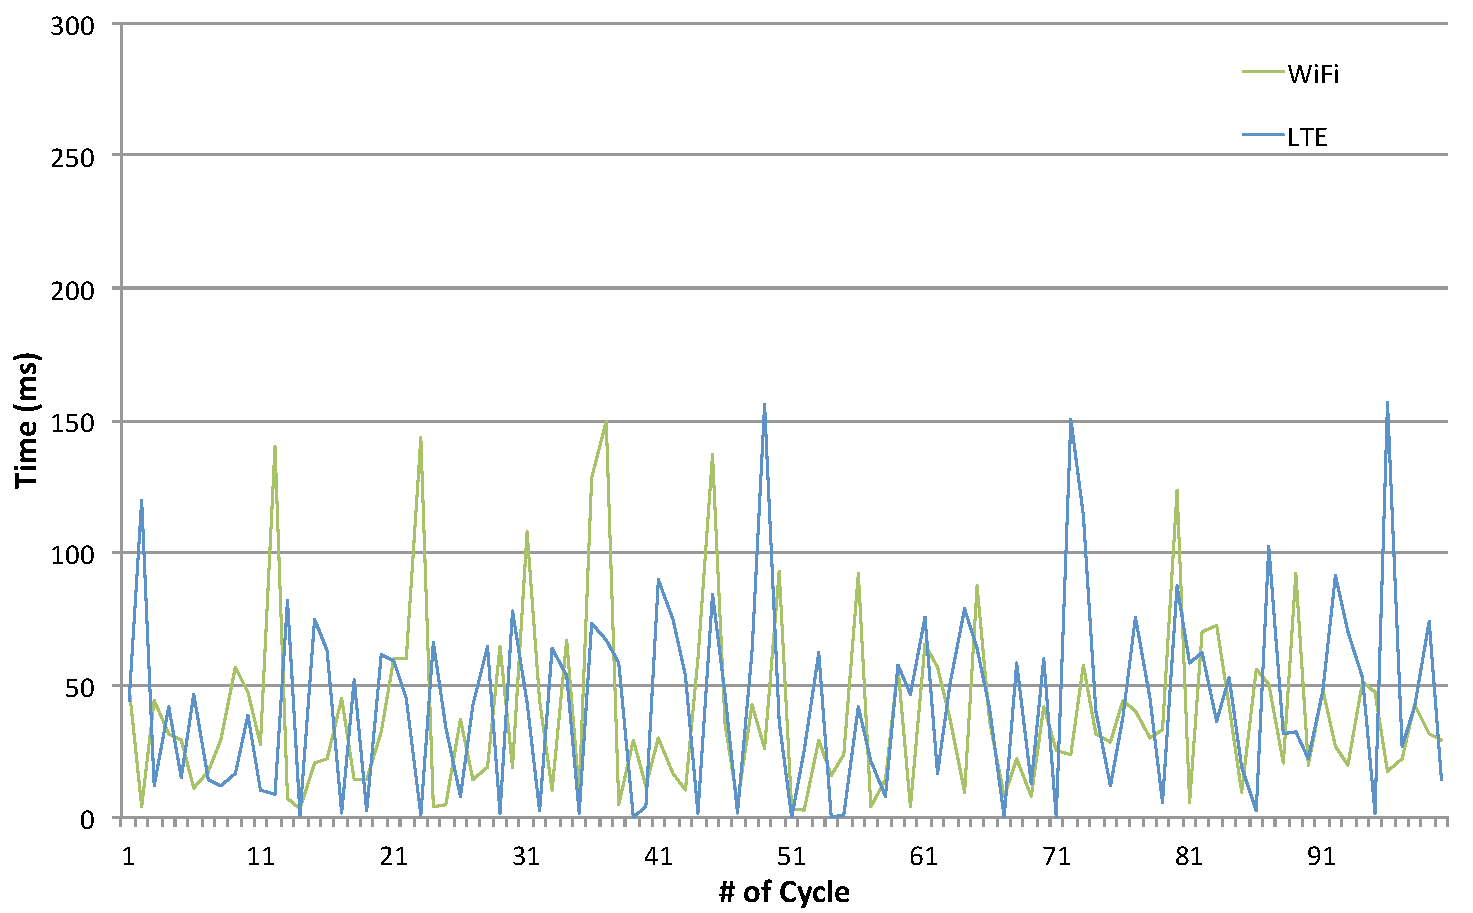
\includegraphics[width=0.8\hsize]{fig/No12_TIPiC_serv_cycle_compare_WiFi_and_LTE.pdf}
 \caption{The periods of image transfers using WiFi and LTE respectively.}
 \label{fig:no12}
\end{figure}

\begin{figure}[!t]
 \centering
 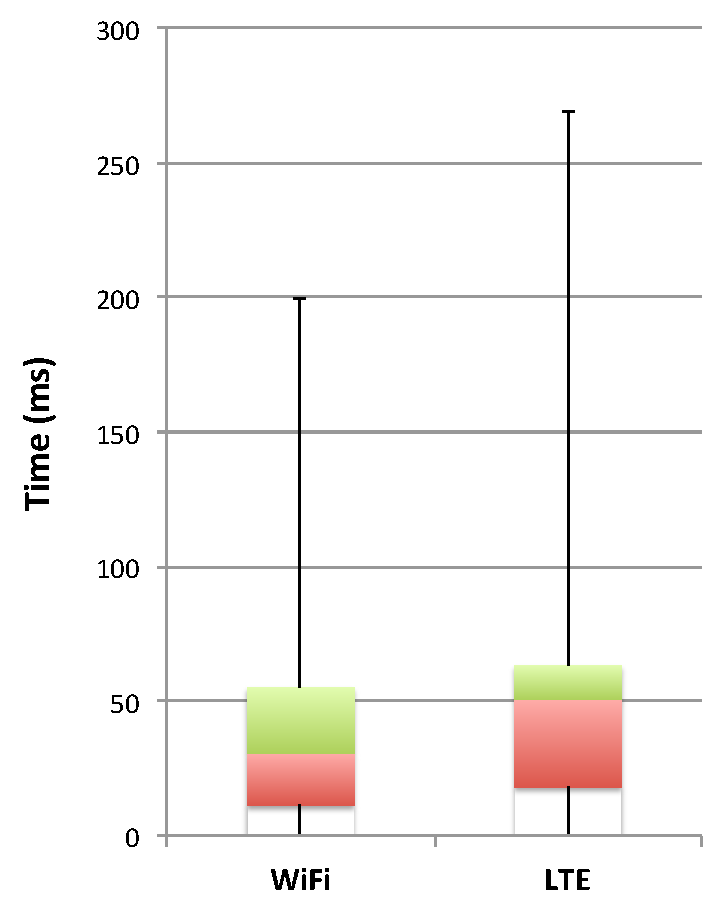
\includegraphics[width=0.5\hsize]{fig/No13_TIPiC_boxplot_compare_WiFi_and_LTE.pdf}
 \caption{Summarized box plotting of the periods for image transfers.}
 \label{fig:no13}
\end{figure}

Fig. \ref{fig:no12} shows a comparison of the periods of image transfers
on a cycle basis for WiFi and LTE.
Fig. \ref{fig:no13} also shows summarized box plotting of these periods.
One can see that the achieved periods of image transfers for WiFi and
LTE exhibit similar characteristics.
Putting together with the result of frame rate shown in
Fig. \ref{fig:no10}, we conclude that WiFi and LTE are competitive to
each other in terms of throughput for image transfers.

\begin{figure}[!t]
 \centering
 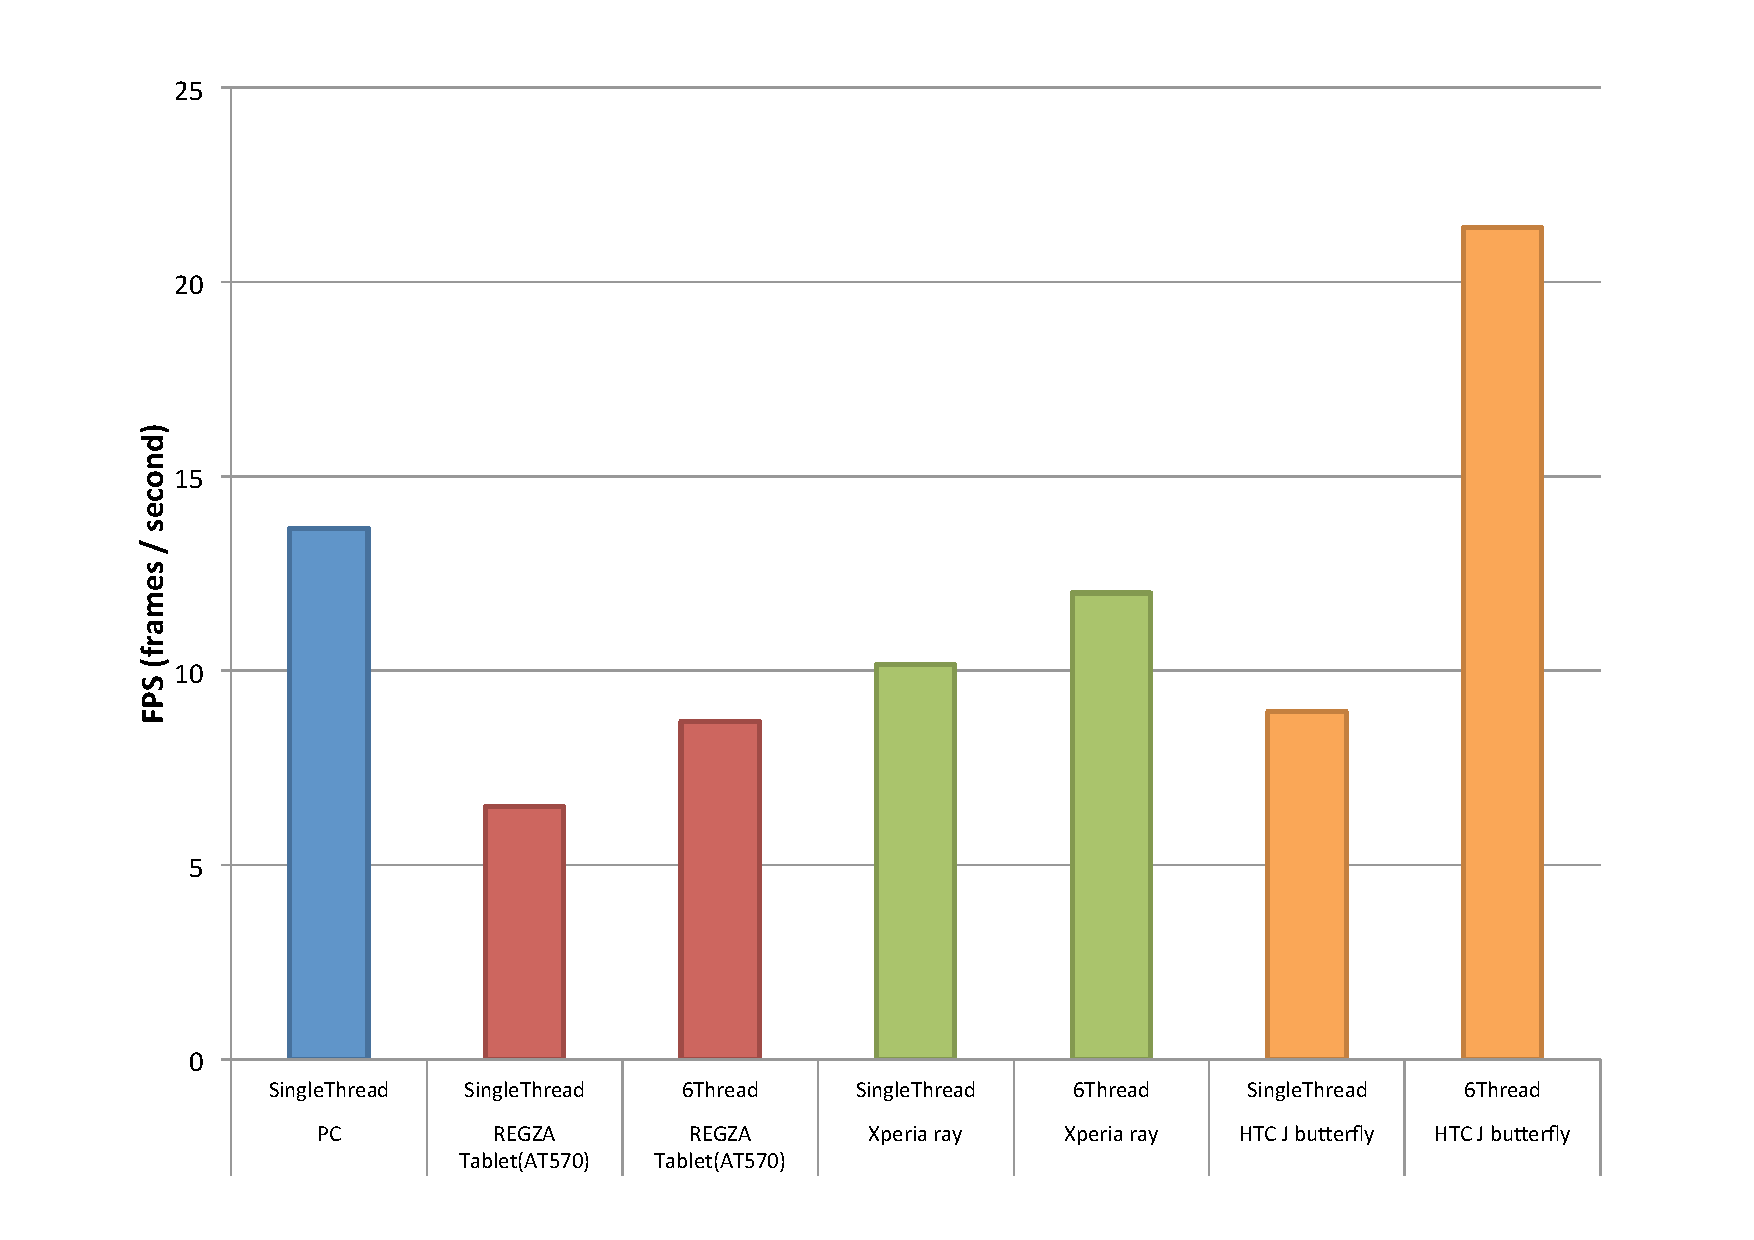
\includegraphics[width=0.8\hsize]{fig/No14_Android_and_PC_benchmarck.pdf}
 \caption{Performance differences among popular Android devices.}
 \label{fig:no14}
\end{figure}

Fig. \ref{fig:no14} shows performance differences among popular Android
devices including Xperia ray (MSM8255@1Ghz, Single Core),
REGZA Tablet (Tegra 3@1.3GHz, Quad Core), and HTC J butterfly Snapdragon
S4 Pro (APQ8064@1.5GHz, Quad Core), when transferring an image of
$640\times480$ pixels.
For a reference, we also plot the performance of a single thread
performing on a laptop PC with an Intel Core i3 processor (3110M@2.4GHz,
Dual Core).
Notably non-trivial performance differences are observed in this
experiment.
Although the class of an employed processor is a primary factor of
performance, we experience that the performance of an equipped camera
also dominates the overall performance of image transfers.
For example, the average number of images per second that the REGZA
Tablet can capture is no more than 11.41, while the Xperia ray and the
HTC J butterfly can capture 23.20 and 25.74 images per second
respectively on average.
Therefore the REGZA Tablet does not exhibit high frame rates for entire
image transfers, even though it employs a rich processor.
Comparing the the Xperia ray and the HTC J butterfly also highlights
that a multicore processor benefits from multithreading more
significantly.
It can be clearly seen that the multithreaded HTC J butterfly even
outperforms the single threaded laptop PC.